% Created by tikzDevice version 0.9 on 2016-01-13 23:39:50
% !TEX encoding = UTF-8 Unicode
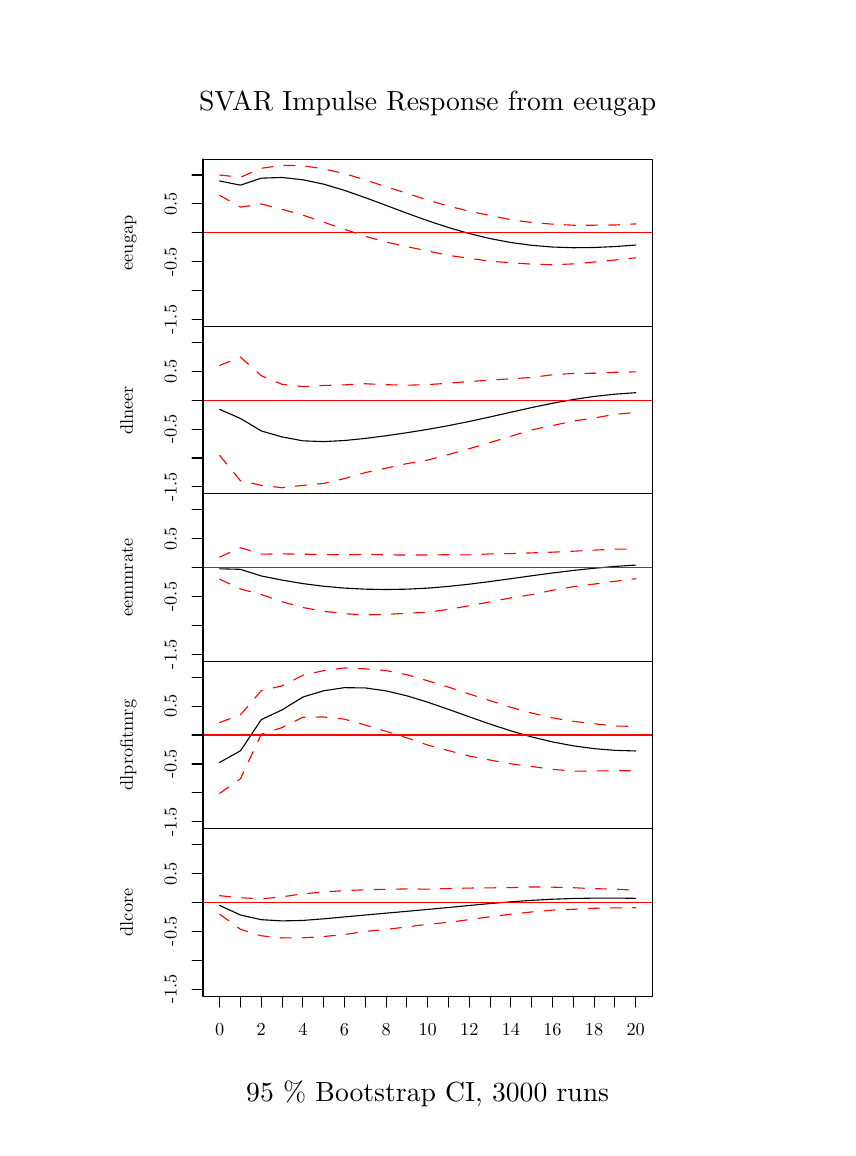
\begin{tikzpicture}[x=1pt,y=1pt]
\definecolor{fillColor}{RGB}{255,255,255}
\path[use as bounding box,fill=fillColor,fill opacity=0.00] (0,0) rectangle (289.08,397.48);
\begin{scope}
\path[clip] ( 63.36,289.48) rectangle (225.72,349.96);
\definecolor{drawColor}{RGB}{0,0,0}

\path[draw=drawColor,line width= 0.4pt,line join=round,line cap=round] ( 69.37,342.09) --
	( 76.89,340.56) --
	( 84.41,343.11) --
	( 91.92,343.34) --
	( 99.44,342.52) --
	(106.96,340.93) --
	(114.47,338.68) --
	(121.99,336.06) --
	(129.51,333.26) --
	(137.02,330.43) --
	(144.54,327.73) --
	(152.06,325.25) --
	(159.57,323.07) --
	(167.09,321.26) --
	(174.61,319.84) --
	(182.12,318.83) --
	(189.64,318.21) --
	(197.16,317.96) --
	(204.67,318.04) --
	(212.19,318.38) --
	(219.71,318.94);
\end{scope}
\begin{scope}
\path[clip] ( 31.68,289.48) rectangle (257.40,349.96);
\definecolor{drawColor}{RGB}{0,0,0}

\node[text=drawColor,anchor=base,inner sep=0pt, outer sep=0pt, scale=  0.66] at (144.54,259.38) {xy{\$}x};

\node[text=drawColor,rotate= 90.00,anchor=base,inner sep=0pt, outer sep=0pt, scale=  0.66] at ( 38.02,319.72) {eeugap};
\end{scope}
\begin{scope}
\path[clip] (  0.00,  0.00) rectangle (289.08,397.48);
\definecolor{drawColor}{RGB}{0,0,0}

\path[draw=drawColor,line width= 0.4pt,line join=round,line cap=round] ( 63.36,292.01) -- ( 63.36,349.97);

\path[draw=drawColor,line width= 0.4pt,line join=round,line cap=round] ( 63.36,292.01) -- ( 59.40,292.01);

\path[draw=drawColor,line width= 0.4pt,line join=round,line cap=round] ( 63.36,302.45) -- ( 59.40,302.45);

\path[draw=drawColor,line width= 0.4pt,line join=round,line cap=round] ( 63.36,312.89) -- ( 59.40,312.89);

\path[draw=drawColor,line width= 0.4pt,line join=round,line cap=round] ( 63.36,323.33) -- ( 59.40,323.33);

\path[draw=drawColor,line width= 0.4pt,line join=round,line cap=round] ( 63.36,333.78) -- ( 59.40,333.78);

\path[draw=drawColor,line width= 0.4pt,line join=round,line cap=round] ( 63.36,344.22) -- ( 59.40,344.22);

\node[text=drawColor,rotate= 90.00,anchor=base,inner sep=0pt, outer sep=0pt, scale=  0.66] at ( 53.86,292.01) {-1.5};

\node[text=drawColor,rotate= 90.00,anchor=base,inner sep=0pt, outer sep=0pt, scale=  0.66] at ( 53.86,312.89) {-0.5};

\node[text=drawColor,rotate= 90.00,anchor=base,inner sep=0pt, outer sep=0pt, scale=  0.66] at ( 53.86,333.78) {0.5};
\end{scope}
\begin{scope}
\path[clip] ( 63.36,289.48) rectangle (225.72,349.96);
\definecolor{drawColor}{RGB}{255,0,0}

\path[draw=drawColor,line width= 0.4pt,line join=round,line cap=round] ( 63.36,323.33) -- (225.72,323.33);

\path[draw=drawColor,line width= 0.4pt,dash pattern=on 4pt off 4pt ,line join=round,line cap=round] ( 69.37,344.23) --
	( 76.89,343.42) --
	( 84.41,346.68) --
	( 91.92,347.72) --
	( 99.44,347.60) --
	(106.96,346.44) --
	(114.47,344.74) --
	(121.99,342.46) --
	(129.51,339.98) --
	(137.02,337.64) --
	(144.54,335.17) --
	(152.06,333.02) --
	(159.57,331.13) --
	(167.09,329.61) --
	(174.61,328.08) --
	(182.12,327.08) --
	(189.64,326.47) --
	(197.16,326.09) --
	(204.67,326.10) --
	(212.19,326.17) --
	(219.71,326.57);

\path[draw=drawColor,line width= 0.4pt,dash pattern=on 4pt off 4pt ,line join=round,line cap=round] ( 69.37,336.88) --
	( 76.89,332.64) --
	( 84.41,333.77) --
	( 91.92,331.83) --
	( 99.44,329.73) --
	(106.96,327.18) --
	(114.47,324.64) --
	(121.99,322.09) --
	(129.51,320.01) --
	(137.02,318.34) --
	(144.54,316.80) --
	(152.06,315.18) --
	(159.57,314.16) --
	(167.09,313.07) --
	(174.61,312.56) --
	(182.12,312.02) --
	(189.64,311.80) --
	(197.16,312.12) --
	(204.67,312.78) --
	(212.19,313.52) --
	(219.71,314.32);
\end{scope}
\begin{scope}
\path[clip] (  0.00,  0.00) rectangle (289.08,397.48);
\definecolor{drawColor}{RGB}{0,0,0}

\path[draw=drawColor,line width= 0.4pt,line join=round,line cap=round] ( 63.36,289.48) --
	(225.72,289.48) --
	(225.72,349.96) --
	( 63.36,349.96) --
	( 63.36,289.48);
\end{scope}
\begin{scope}
\path[clip] ( 63.36,228.99) rectangle (225.72,289.48);
\definecolor{drawColor}{RGB}{0,0,0}

\path[draw=drawColor,line width= 0.4pt,line join=round,line cap=round] ( 69.37,259.56) --
	( 76.89,256.26) --
	( 84.41,251.75) --
	( 91.92,249.60) --
	( 99.44,248.18) --
	(106.96,247.91) --
	(114.47,248.29) --
	(121.99,249.06) --
	(129.51,250.02) --
	(137.02,251.11) --
	(144.54,252.32) --
	(152.06,253.67) --
	(159.57,255.18) --
	(167.09,256.82) --
	(174.61,258.52) --
	(182.12,260.20) --
	(189.64,261.76) --
	(197.16,263.11) --
	(204.67,264.22) --
	(212.19,265.04) --
	(219.71,265.58);
\end{scope}
\begin{scope}
\path[clip] ( 31.68,228.99) rectangle (257.40,289.48);
\definecolor{drawColor}{RGB}{0,0,0}

\node[text=drawColor,anchor=base,inner sep=0pt, outer sep=0pt, scale=  0.66] at (144.54,198.89) {xy{\$}x};

\node[text=drawColor,rotate= 90.00,anchor=base,inner sep=0pt, outer sep=0pt, scale=  0.66] at ( 38.02,259.23) {dlneer};
\end{scope}
\begin{scope}
\path[clip] (  0.00,  0.00) rectangle (289.08,397.48);
\definecolor{drawColor}{RGB}{0,0,0}

\path[draw=drawColor,line width= 0.4pt,line join=round,line cap=round] ( 63.36,231.52) -- ( 63.36,289.48);

\path[draw=drawColor,line width= 0.4pt,line join=round,line cap=round] ( 63.36,231.52) -- ( 59.40,231.52);

\path[draw=drawColor,line width= 0.4pt,line join=round,line cap=round] ( 63.36,241.96) -- ( 59.40,241.96);

\path[draw=drawColor,line width= 0.4pt,line join=round,line cap=round] ( 63.36,252.40) -- ( 59.40,252.40);

\path[draw=drawColor,line width= 0.4pt,line join=round,line cap=round] ( 63.36,262.85) -- ( 59.40,262.85);

\path[draw=drawColor,line width= 0.4pt,line join=round,line cap=round] ( 63.36,273.29) -- ( 59.40,273.29);

\path[draw=drawColor,line width= 0.4pt,line join=round,line cap=round] ( 63.36,283.73) -- ( 59.40,283.73);

\node[text=drawColor,rotate= 90.00,anchor=base,inner sep=0pt, outer sep=0pt, scale=  0.66] at ( 53.86,231.52) {-1.5};

\node[text=drawColor,rotate= 90.00,anchor=base,inner sep=0pt, outer sep=0pt, scale=  0.66] at ( 53.86,252.40) {-0.5};

\node[text=drawColor,rotate= 90.00,anchor=base,inner sep=0pt, outer sep=0pt, scale=  0.66] at ( 53.86,273.29) {0.5};
\end{scope}
\begin{scope}
\path[clip] ( 63.36,228.99) rectangle (225.72,289.48);
\definecolor{drawColor}{RGB}{255,0,0}

\path[draw=drawColor,line width= 0.4pt,line join=round,line cap=round] ( 63.36,262.85) -- (225.72,262.85);

\path[draw=drawColor,line width= 0.4pt,dash pattern=on 4pt off 4pt ,line join=round,line cap=round] ( 69.37,275.42) --
	( 76.89,278.43) --
	( 84.41,271.69) --
	( 91.92,268.61) --
	( 99.44,267.77) --
	(106.96,268.19) --
	(114.47,268.40) --
	(121.99,268.80) --
	(129.51,268.47) --
	(137.02,268.28) --
	(144.54,268.49) --
	(152.06,269.01) --
	(159.57,269.61) --
	(167.09,270.13) --
	(174.61,270.60) --
	(182.12,271.09) --
	(189.64,272.07) --
	(197.16,272.52) --
	(204.67,272.60) --
	(212.19,272.96) --
	(219.71,273.10);

\path[draw=drawColor,line width= 0.4pt,dash pattern=on 4pt off 4pt ,line join=round,line cap=round] ( 69.37,242.92) --
	( 76.89,233.75) --
	( 84.41,232.11) --
	( 91.92,231.23) --
	( 99.44,232.08) --
	(106.96,232.79) --
	(114.47,234.54) --
	(121.99,236.71) --
	(129.51,238.30) --
	(137.02,239.95) --
	(144.54,241.23) --
	(152.06,243.23) --
	(159.57,245.34) --
	(167.09,247.57) --
	(174.61,249.83) --
	(182.12,252.14) --
	(189.64,253.71) --
	(197.16,255.32) --
	(204.67,256.43) --
	(212.19,257.74) --
	(219.71,258.45);
\end{scope}
\begin{scope}
\path[clip] (  0.00,  0.00) rectangle (289.08,397.48);
\definecolor{drawColor}{RGB}{0,0,0}

\path[draw=drawColor,line width= 0.4pt,line join=round,line cap=round] ( 63.36,228.99) --
	(225.72,228.99) --
	(225.72,289.48) --
	( 63.36,289.48) --
	( 63.36,228.99);
\end{scope}
\begin{scope}
\path[clip] ( 63.36,168.50) rectangle (225.72,228.99);
\definecolor{drawColor}{RGB}{0,0,0}

\path[draw=drawColor,line width= 0.4pt,line join=round,line cap=round] ( 69.37,201.94) --
	( 76.89,201.75) --
	( 84.41,199.35) --
	( 91.92,197.86) --
	( 99.44,196.59) --
	(106.96,195.63) --
	(114.47,194.97) --
	(121.99,194.58) --
	(129.51,194.45) --
	(137.02,194.58) --
	(144.54,194.96) --
	(152.06,195.58) --
	(159.57,196.39) --
	(167.09,197.34) --
	(174.61,198.37) --
	(182.12,199.42) --
	(189.64,200.43) --
	(197.16,201.34) --
	(204.67,202.14) --
	(212.19,202.79) --
	(219.71,203.29);
\end{scope}
\begin{scope}
\path[clip] ( 31.68,168.50) rectangle (257.40,228.99);
\definecolor{drawColor}{RGB}{0,0,0}

\node[text=drawColor,anchor=base,inner sep=0pt, outer sep=0pt, scale=  0.66] at (144.54,138.40) {xy{\$}x};

\node[text=drawColor,rotate= 90.00,anchor=base,inner sep=0pt, outer sep=0pt, scale=  0.66] at ( 38.02,198.74) {eemmrate};
\end{scope}
\begin{scope}
\path[clip] (  0.00,  0.00) rectangle (289.08,397.48);
\definecolor{drawColor}{RGB}{0,0,0}

\path[draw=drawColor,line width= 0.4pt,line join=round,line cap=round] ( 63.36,171.03) -- ( 63.36,228.99);

\path[draw=drawColor,line width= 0.4pt,line join=round,line cap=round] ( 63.36,171.03) -- ( 59.40,171.03);

\path[draw=drawColor,line width= 0.4pt,line join=round,line cap=round] ( 63.36,181.47) -- ( 59.40,181.47);

\path[draw=drawColor,line width= 0.4pt,line join=round,line cap=round] ( 63.36,191.91) -- ( 59.40,191.91);

\path[draw=drawColor,line width= 0.4pt,line join=round,line cap=round] ( 63.36,202.36) -- ( 59.40,202.36);

\path[draw=drawColor,line width= 0.4pt,line join=round,line cap=round] ( 63.36,212.80) -- ( 59.40,212.80);

\path[draw=drawColor,line width= 0.4pt,line join=round,line cap=round] ( 63.36,223.24) -- ( 59.40,223.24);

\node[text=drawColor,rotate= 90.00,anchor=base,inner sep=0pt, outer sep=0pt, scale=  0.66] at ( 53.86,171.03) {-1.5};

\node[text=drawColor,rotate= 90.00,anchor=base,inner sep=0pt, outer sep=0pt, scale=  0.66] at ( 53.86,191.91) {-0.5};

\node[text=drawColor,rotate= 90.00,anchor=base,inner sep=0pt, outer sep=0pt, scale=  0.66] at ( 53.86,212.80) {0.5};
\end{scope}
\begin{scope}
\path[clip] ( 63.36,168.50) rectangle (225.72,228.99);
\definecolor{drawColor}{RGB}{255,0,0}

\path[draw=drawColor,line width= 0.4pt,line join=round,line cap=round] ( 63.36,202.36) -- (225.72,202.36);

\path[draw=drawColor,line width= 0.4pt,dash pattern=on 4pt off 4pt ,line join=round,line cap=round] ( 69.37,206.18) --
	( 76.89,209.57) --
	( 84.41,207.24) --
	( 91.92,207.33) --
	( 99.44,207.21) --
	(106.96,207.11) --
	(114.47,206.97) --
	(121.99,207.17) --
	(129.51,206.99) --
	(137.02,206.90) --
	(144.54,206.92) --
	(152.06,207.04) --
	(159.57,206.96) --
	(167.09,207.33) --
	(174.61,207.43) --
	(182.12,207.69) --
	(189.64,207.95) --
	(197.16,208.29) --
	(204.67,208.69) --
	(212.19,209.04) --
	(219.71,209.02);

\path[draw=drawColor,line width= 0.4pt,dash pattern=on 4pt off 4pt ,line join=round,line cap=round] ( 69.37,198.19) --
	( 76.89,194.65) --
	( 84.41,192.64) --
	( 91.92,190.03) --
	( 99.44,187.94) --
	(106.96,186.62) --
	(114.47,185.71) --
	(121.99,185.30) --
	(129.51,185.46) --
	(137.02,185.87) --
	(144.54,186.26) --
	(152.06,187.28) --
	(159.57,188.59) --
	(167.09,189.99) --
	(174.61,191.44) --
	(182.12,192.61) --
	(189.64,194.19) --
	(197.16,195.46) --
	(204.67,196.42) --
	(212.19,197.43) --
	(219.71,198.36);
\end{scope}
\begin{scope}
\path[clip] (  0.00,  0.00) rectangle (289.08,397.48);
\definecolor{drawColor}{RGB}{0,0,0}

\path[draw=drawColor,line width= 0.4pt,line join=round,line cap=round] ( 63.36,168.50) --
	(225.72,168.50) --
	(225.72,228.99) --
	( 63.36,228.99) --
	( 63.36,168.50);
\end{scope}
\begin{scope}
\path[clip] ( 63.36,108.01) rectangle (225.72,168.50);
\definecolor{drawColor}{RGB}{0,0,0}

\path[draw=drawColor,line width= 0.4pt,line join=round,line cap=round] ( 69.37,131.98) --
	( 76.89,136.17) --
	( 84.41,147.45) --
	( 91.92,150.96) --
	( 99.44,155.60) --
	(106.96,157.87) --
	(114.47,158.99) --
	(121.99,158.89) --
	(129.51,157.83) --
	(137.02,156.04) --
	(144.54,153.74) --
	(152.06,151.15) --
	(159.57,148.46) --
	(167.09,145.82) --
	(174.61,143.37) --
	(182.12,141.20) --
	(189.64,139.39) --
	(197.16,137.97) --
	(204.67,136.96) --
	(212.19,136.35) --
	(219.71,136.11);
\end{scope}
\begin{scope}
\path[clip] ( 31.68,108.01) rectangle (257.40,168.50);
\definecolor{drawColor}{RGB}{0,0,0}

\node[text=drawColor,anchor=base,inner sep=0pt, outer sep=0pt, scale=  0.66] at (144.54, 77.91) {xy{\$}x};

\node[text=drawColor,rotate= 90.00,anchor=base,inner sep=0pt, outer sep=0pt, scale=  0.66] at ( 38.02,138.25) {dlprofitmrg};
\end{scope}
\begin{scope}
\path[clip] (  0.00,  0.00) rectangle (289.08,397.48);
\definecolor{drawColor}{RGB}{0,0,0}

\path[draw=drawColor,line width= 0.4pt,line join=round,line cap=round] ( 63.36,110.54) -- ( 63.36,168.50);

\path[draw=drawColor,line width= 0.4pt,line join=round,line cap=round] ( 63.36,110.54) -- ( 59.40,110.54);

\path[draw=drawColor,line width= 0.4pt,line join=round,line cap=round] ( 63.36,120.98) -- ( 59.40,120.98);

\path[draw=drawColor,line width= 0.4pt,line join=round,line cap=round] ( 63.36,131.42) -- ( 59.40,131.42);

\path[draw=drawColor,line width= 0.4pt,line join=round,line cap=round] ( 63.36,141.87) -- ( 59.40,141.87);

\path[draw=drawColor,line width= 0.4pt,line join=round,line cap=round] ( 63.36,152.31) -- ( 59.40,152.31);

\path[draw=drawColor,line width= 0.4pt,line join=round,line cap=round] ( 63.36,162.75) -- ( 59.40,162.75);

\node[text=drawColor,rotate= 90.00,anchor=base,inner sep=0pt, outer sep=0pt, scale=  0.66] at ( 53.86,110.54) {-1.5};

\node[text=drawColor,rotate= 90.00,anchor=base,inner sep=0pt, outer sep=0pt, scale=  0.66] at ( 53.86,131.42) {-0.5};

\node[text=drawColor,rotate= 90.00,anchor=base,inner sep=0pt, outer sep=0pt, scale=  0.66] at ( 53.86,152.31) {0.5};
\end{scope}
\begin{scope}
\path[clip] ( 63.36,108.01) rectangle (225.72,168.50);
\definecolor{drawColor}{RGB}{255,0,0}

\path[draw=drawColor,line width= 0.4pt,line join=round,line cap=round] ( 63.36,141.87) -- (225.72,141.87);

\path[draw=drawColor,line width= 0.4pt,dash pattern=on 4pt off 4pt ,line join=round,line cap=round] ( 69.37,146.40) --
	( 76.89,149.16) --
	( 84.41,157.93) --
	( 91.92,159.63) --
	( 99.44,163.48) --
	(106.96,165.14) --
	(114.47,166.11) --
	(121.99,165.81) --
	(129.51,165.16) --
	(137.02,163.67) --
	(144.54,161.47) --
	(152.06,159.20) --
	(159.57,156.69) --
	(167.09,154.30) --
	(174.61,151.87) --
	(182.12,149.81) --
	(189.64,148.07) --
	(197.16,146.83) --
	(204.67,145.95) --
	(212.19,145.14) --
	(219.71,144.99);

\path[draw=drawColor,line width= 0.4pt,dash pattern=on 4pt off 4pt ,line join=round,line cap=round] ( 69.37,120.78) --
	( 76.89,126.08) --
	( 84.41,142.17) --
	( 91.92,144.57) --
	( 99.44,148.31) --
	(106.96,148.39) --
	(114.47,147.60) --
	(121.99,145.48) --
	(129.51,143.22) --
	(137.02,140.84) --
	(144.54,138.25) --
	(152.06,136.25) --
	(159.57,134.27) --
	(167.09,132.83) --
	(174.61,131.46) --
	(182.12,130.51) --
	(189.64,129.48) --
	(197.16,128.80) --
	(204.67,128.90) --
	(212.19,128.95) --
	(219.71,128.96);
\end{scope}
\begin{scope}
\path[clip] (  0.00,  0.00) rectangle (289.08,397.48);
\definecolor{drawColor}{RGB}{0,0,0}

\path[draw=drawColor,line width= 0.4pt,line join=round,line cap=round] ( 63.36,108.01) --
	(225.72,108.01) --
	(225.72,168.50) --
	( 63.36,168.50) --
	( 63.36,108.01);
\end{scope}
\begin{scope}
\path[clip] ( 63.36, 47.52) rectangle (225.72,108.01);
\definecolor{drawColor}{RGB}{0,0,0}

\path[draw=drawColor,line width= 0.4pt,line join=round,line cap=round] ( 69.37, 80.30) --
	( 76.89, 76.85) --
	( 84.41, 75.15) --
	( 91.92, 74.71) --
	( 99.44, 74.88) --
	(106.96, 75.46) --
	(114.47, 76.15) --
	(121.99, 76.84) --
	(129.51, 77.51) --
	(137.02, 78.17) --
	(144.54, 78.85) --
	(152.06, 79.56) --
	(159.57, 80.28) --
	(167.09, 80.98) --
	(174.61, 81.61) --
	(182.12, 82.14) --
	(189.64, 82.55) --
	(197.16, 82.81) --
	(204.67, 82.94) --
	(212.19, 82.96) --
	(219.71, 82.87);
\end{scope}
\begin{scope}
\path[clip] ( 31.68, 47.52) rectangle (257.40,108.01);
\definecolor{drawColor}{RGB}{0,0,0}

\node[text=drawColor,anchor=base,inner sep=0pt, outer sep=0pt, scale=  0.66] at (144.54, 17.42) {xy{\$}x};

\node[text=drawColor,rotate= 90.00,anchor=base,inner sep=0pt, outer sep=0pt, scale=  0.66] at ( 38.02, 77.76) {dlcore};
\end{scope}
\begin{scope}
\path[clip] (  0.00,  0.00) rectangle (289.08,397.48);
\definecolor{drawColor}{RGB}{0,0,0}

\path[draw=drawColor,line width= 0.4pt,line join=round,line cap=round] ( 63.36, 50.05) -- ( 63.36,108.01);

\path[draw=drawColor,line width= 0.4pt,line join=round,line cap=round] ( 63.36, 50.05) -- ( 59.40, 50.05);

\path[draw=drawColor,line width= 0.4pt,line join=round,line cap=round] ( 63.36, 60.49) -- ( 59.40, 60.49);

\path[draw=drawColor,line width= 0.4pt,line join=round,line cap=round] ( 63.36, 70.94) -- ( 59.40, 70.94);

\path[draw=drawColor,line width= 0.4pt,line join=round,line cap=round] ( 63.36, 81.38) -- ( 59.40, 81.38);

\path[draw=drawColor,line width= 0.4pt,line join=round,line cap=round] ( 63.36, 91.82) -- ( 59.40, 91.82);

\path[draw=drawColor,line width= 0.4pt,line join=round,line cap=round] ( 63.36,102.26) -- ( 59.40,102.26);

\node[text=drawColor,rotate= 90.00,anchor=base,inner sep=0pt, outer sep=0pt, scale=  0.66] at ( 53.86, 50.05) {-1.5};

\node[text=drawColor,rotate= 90.00,anchor=base,inner sep=0pt, outer sep=0pt, scale=  0.66] at ( 53.86, 70.94) {-0.5};

\node[text=drawColor,rotate= 90.00,anchor=base,inner sep=0pt, outer sep=0pt, scale=  0.66] at ( 53.86, 91.82) {0.5};

\path[draw=drawColor,line width= 0.4pt,line join=round,line cap=round] ( 69.37, 47.52) -- (219.71, 47.52);

\path[draw=drawColor,line width= 0.4pt,line join=round,line cap=round] ( 69.37, 47.52) -- ( 69.37, 43.56);

\path[draw=drawColor,line width= 0.4pt,line join=round,line cap=round] ( 76.89, 47.52) -- ( 76.89, 43.56);

\path[draw=drawColor,line width= 0.4pt,line join=round,line cap=round] ( 84.41, 47.52) -- ( 84.41, 43.56);

\path[draw=drawColor,line width= 0.4pt,line join=round,line cap=round] ( 91.92, 47.52) -- ( 91.92, 43.56);

\path[draw=drawColor,line width= 0.4pt,line join=round,line cap=round] ( 99.44, 47.52) -- ( 99.44, 43.56);

\path[draw=drawColor,line width= 0.4pt,line join=round,line cap=round] (106.96, 47.52) -- (106.96, 43.56);

\path[draw=drawColor,line width= 0.4pt,line join=round,line cap=round] (114.47, 47.52) -- (114.47, 43.56);

\path[draw=drawColor,line width= 0.4pt,line join=round,line cap=round] (121.99, 47.52) -- (121.99, 43.56);

\path[draw=drawColor,line width= 0.4pt,line join=round,line cap=round] (129.51, 47.52) -- (129.51, 43.56);

\path[draw=drawColor,line width= 0.4pt,line join=round,line cap=round] (137.02, 47.52) -- (137.02, 43.56);

\path[draw=drawColor,line width= 0.4pt,line join=round,line cap=round] (144.54, 47.52) -- (144.54, 43.56);

\path[draw=drawColor,line width= 0.4pt,line join=round,line cap=round] (152.06, 47.52) -- (152.06, 43.56);

\path[draw=drawColor,line width= 0.4pt,line join=round,line cap=round] (159.57, 47.52) -- (159.57, 43.56);

\path[draw=drawColor,line width= 0.4pt,line join=round,line cap=round] (167.09, 47.52) -- (167.09, 43.56);

\path[draw=drawColor,line width= 0.4pt,line join=round,line cap=round] (174.61, 47.52) -- (174.61, 43.56);

\path[draw=drawColor,line width= 0.4pt,line join=round,line cap=round] (182.12, 47.52) -- (182.12, 43.56);

\path[draw=drawColor,line width= 0.4pt,line join=round,line cap=round] (189.64, 47.52) -- (189.64, 43.56);

\path[draw=drawColor,line width= 0.4pt,line join=round,line cap=round] (197.16, 47.52) -- (197.16, 43.56);

\path[draw=drawColor,line width= 0.4pt,line join=round,line cap=round] (204.67, 47.52) -- (204.67, 43.56);

\path[draw=drawColor,line width= 0.4pt,line join=round,line cap=round] (212.19, 47.52) -- (212.19, 43.56);

\path[draw=drawColor,line width= 0.4pt,line join=round,line cap=round] (219.71, 47.52) -- (219.71, 43.56);

\node[text=drawColor,anchor=base,inner sep=0pt, outer sep=0pt, scale=  0.66] at ( 69.37, 33.26) {0};

\node[text=drawColor,anchor=base,inner sep=0pt, outer sep=0pt, scale=  0.66] at ( 84.41, 33.26) {2};

\node[text=drawColor,anchor=base,inner sep=0pt, outer sep=0pt, scale=  0.66] at ( 99.44, 33.26) {4};

\node[text=drawColor,anchor=base,inner sep=0pt, outer sep=0pt, scale=  0.66] at (114.47, 33.26) {6};

\node[text=drawColor,anchor=base,inner sep=0pt, outer sep=0pt, scale=  0.66] at (129.51, 33.26) {8};

\node[text=drawColor,anchor=base,inner sep=0pt, outer sep=0pt, scale=  0.66] at (144.54, 33.26) {10};

\node[text=drawColor,anchor=base,inner sep=0pt, outer sep=0pt, scale=  0.66] at (159.57, 33.26) {12};

\node[text=drawColor,anchor=base,inner sep=0pt, outer sep=0pt, scale=  0.66] at (174.61, 33.26) {14};

\node[text=drawColor,anchor=base,inner sep=0pt, outer sep=0pt, scale=  0.66] at (189.64, 33.26) {16};

\node[text=drawColor,anchor=base,inner sep=0pt, outer sep=0pt, scale=  0.66] at (204.67, 33.26) {18};

\node[text=drawColor,anchor=base,inner sep=0pt, outer sep=0pt, scale=  0.66] at (219.71, 33.26) {20};

\path[draw=drawColor,line width= 0.4pt,line join=round,line cap=round] ( 63.36, 47.52) --
	(225.72, 47.52) --
	(225.72,108.01) --
	( 63.36,108.01) --
	( 63.36, 47.52);
\end{scope}
\begin{scope}
\path[clip] ( 63.36, 47.52) rectangle (225.72,108.01);
\definecolor{drawColor}{RGB}{255,0,0}

\path[draw=drawColor,line width= 0.4pt,line join=round,line cap=round] ( 63.36, 81.38) -- (225.72, 81.38);

\path[draw=drawColor,line width= 0.4pt,dash pattern=on 4pt off 4pt ,line join=round,line cap=round] ( 69.37, 83.81) --
	( 76.89, 83.08) --
	( 84.41, 82.68) --
	( 91.92, 83.41) --
	( 99.44, 84.48) --
	(106.96, 85.16) --
	(114.47, 85.65) --
	(121.99, 85.96) --
	(129.51, 86.13) --
	(137.02, 86.27) --
	(144.54, 86.19) --
	(152.06, 86.42) --
	(159.57, 86.57) --
	(167.09, 86.65) --
	(174.61, 86.74) --
	(182.12, 86.98) --
	(189.64, 86.90) --
	(197.16, 86.69) --
	(204.67, 86.36) --
	(212.19, 86.20) --
	(219.71, 85.76);

\path[draw=drawColor,line width= 0.4pt,dash pattern=on 4pt off 4pt ,line join=round,line cap=round] ( 69.37, 77.15) --
	( 76.89, 71.66) --
	( 84.41, 69.33) --
	( 91.92, 68.55) --
	( 99.44, 68.59) --
	(106.96, 69.06) --
	(114.47, 69.79) --
	(121.99, 70.92) --
	(129.51, 71.63) --
	(137.02, 72.54) --
	(144.54, 73.50) --
	(152.06, 74.19) --
	(159.57, 75.19) --
	(167.09, 76.21) --
	(174.61, 77.12) --
	(182.12, 77.95) --
	(189.64, 78.60) --
	(197.16, 78.92) --
	(204.67, 79.28) --
	(212.19, 79.42) --
	(219.71, 79.48);
\end{scope}
\begin{scope}
\path[clip] (  0.00,  0.00) rectangle (289.08,397.48);
\definecolor{drawColor}{RGB}{0,0,0}

\node[text=drawColor,anchor=base,inner sep=0pt, outer sep=0pt, scale=  1.00] at (144.54,367.39) {SVAR Impulse Response from eeugap};

\node[text=drawColor,anchor=base,inner sep=0pt, outer sep=0pt, scale=  1.00] at (144.54,  9.50) {95 {\%} Bootstrap CI,  3000 runs};
\end{scope}
\end{tikzpicture}
